% THIS IS SIGPROC-SP.TEX - VERSION 3.1
% WORKS WITH V3.2SP OF ACM_PROC_ARTICLE-SP.CLS
% APRIL 2009
%
% It is an example file showing how to use the 'acm_proc_article-sp.cls' V3.2SP
% LaTeX2e document class file for Conference Proceedings submissions.
% ----------------------------------------------------------------------------------------------------------------
% This .tex file (and associated .cls V3.2SP) *DOES NOT* produce:
%       1) The Permission Statement
%       2) The Conference (location) Info information
%       3) The Copyright Line with ACM data
%       4) Page numbering
% ---------------------------------------------------------------------------------------------------------------
% It is an example which *does* use the .bib file (from which the .bbl file
% is produced).
% REMEMBER HOWEVER: After having produced the .bbl file,
% and prior to final submission,
% you need to 'insert'  your .bbl file into your source .tex file so as to provide
% ONE 'self-contained' source file.
%
% Questions regarding SIGS should be sent to
% Adrienne Griscti ---> griscti@acm.org
%
% Questions/suggestions regarding the guidelines, .tex and .cls files, etc. to
% Gerald Murray ---> murray@hq.acm.org
%
% For tracking purposes - this is V3.1SP - APRIL 2009

\documentclass{acm_proc_article-sp}
\usepackage{algorithm}
\usepackage{algorithmicx}
\usepackage[noend]{algpseudocode}
\algrenewcomment[1]{\(\triangleright\) #1}
\usepackage{hyperref}
\usepackage[table]{xcolor}


\DeclareMathOperator*{\argmax}{arg\,max}
\DeclareMathOperator*{\argmin}{arg\,min}


\begin{document}

\title{Data Fusion Using Source Trustworthiness}
%
% You need the command \numberofauthors to handle the 'placement
% and alignment' of the authors beneath the title.
%
% For aesthetic reasons, we recommend 'three authors at a time'
% i.e. three 'name/affiliation blocks' be placed beneath the title.
%
% NOTE: You are NOT restricted in how many 'rows' of
% "name/affiliations" may appear. We just ask that you restrict
% the number of 'columns' to three.
%
% Because of the available 'opening page real-estate'
% we ask you to refrain from putting more than six authors
% (two rows with three columns) beneath the article title.
% More than six makes the first-page appear very cluttered indeed.
%
% Use the \alignauthor commands to handle the names
% and affiliations for an 'aesthetic maximum' of six authors.
% Add names, affiliations, addresses for
% the seventh etc. author(s) as the argument for the
% \additionalauthors command.
% These 'additional authors' will be output/set for you
% without further effort on your part as the last section in
% the body of your article BEFORE References or any Appendices.

\numberofauthors{3} %  in this sample file, there are a *total*
% of EIGHT authors. SIX appear on the 'first-page' (for formatting
% reasons) and the remaining two appear in the \additionalauthors section.
%
\author{
% You can go ahead and credit any number of authors here,
% e.g. one 'row of three' or two rows (consisting of one row of three
% and a second row of one, two or three).
%
% The command \alignauthor (no curly braces needed) should
% precede each author name, affiliation/snail-mail address and
% e-mail address. Additionally, tag each line of
% affiliation/address with \affaddr, and tag the
% e-mail address with \email.
%
% 1st. author
\alignauthor
Manual Heinkel \\
       \affaddr{UMass Amherst}\\
       \affaddr{140 Governors Drive}\\
       \affaddr{Amherst, Massachusetts}\\
       \email{heinkel@cs.umass.edu}
% 2nd. author
\alignauthor
Nicholas Monath \\
       \affaddr{UMass Amherst}\\
       \affaddr{140 Governors Drive}\\
       \affaddr{Amherst, Massachusetts}\\
       \email{nmonath@cs.umass.edu}
% 3rd. author
\alignauthor 
Lakshmi Nair \\
       \affaddr{UMass Amherst}\\
       \affaddr{140 Governors Drive}\\
       \affaddr{Amherst, Massachusetts}\\
       \email{lvnair@cs.umass.edu}
}
\date{8 March 2015}
% Just remember to make sure that the TOTAL number of authors
% is the number that will appear on the first page PLUS the
% number that will appear in the \additionalauthors section.

\maketitle


% A category with the (minimum) three required fields
%\category{H.4}{Information Systems Applications}{Miscellaneous}
%A category including the fourth, optional field follows...
%\category{D.2.8}{Software Engineering}{Metrics}[complexity measures, performance measures]

%\terms{Theory}

%\keywords{ACM proceedings, \LaTeX, text tagging} % NOT required for Proceedings

\section{Introduction}

The advent of data sources on the web in the last two decades has sparked the need for automated methods of combining sources into a single source. As these data sources often contain noisy and incorrect data, techniques for discerning the correct value among a set of conflicting values must be developed. These techniques solve the problem of data fusion. In data fusion, we consider information or $attributes$ of $entities$ provided by various $sources$. The entities include companies, airplane flights, books etc and attributes for these entities include open and close prices, time delays and isbn numbers respectively. Data sources include any site or database on the web. Data fusion is challenging in that the data may be stored in a variety of formats. Values for an entity's attributes may be semantically equivalent without having the same representation (e.g \$104Mil and 104,000,000 as a company's holding or Ernest Hemingway and E. Hemingway as the author of a book). In certain cases, the range of values for an attribute is not known. The decision of selecting the correct value for an attribute must be made under a great deal of uncertainty in a situation that is heavily domain dependent. Typically, no prior knowledge is known about the authenticity of the data sources. Labeled data is scarce and so supervised methods for data fusion are not practical. Most approaches to data fusion are unsupervised and make use of algorithms such as Expectation-Maximization (EM). A further difficulty is that the causes of erroneous data cannot easily be modeled by common distributions. Many of the current approaches to data fusion in the literature currently focus on modeling the trustworthiness of a data source. However, it is possible that a data source reliably provides values for one attribute, but not others. For example, Orbitz might accurately provide the departure time of a flight while frequently providing an incorrect value for the delay of a flight. In this work, we present models of the trustworthiness each attribute provided by a source. Attributes of entities are often assumed to be independent. We propose a possible model which captures the trustworthiness of sources as well as dependence among attributes.  Other methods in the literature model copying between data sources and the variance of the attributes. Few approaches consider all of these well studied features. We hope to investigate if we can come up with a model which covers all of these features. 

\section{Related Work}
Data fusion is also referred to as truth discovery \cite{waguih:truth} \cite{yin:truth} and data integration \cite{sarma:data} \cite{zhao:bayesian}. While there has been some work on how data fusion pertains to information extraction, specifically question answering \cite{wu:corroborating}, the significant body of literature pertains to the construction of databases, particularly relational databases and, recently, knowledge bases \cite{dong:data}. 



The problem of data fusion in relational databases typically consists of multiple phases \cite{bleiholder:data} \cite{li:truth}. Given a collection of data sources, which all contain data that is to be stored in a particular relation, the first step is often the mapping of the data sources' schema to the schema of the underlying relation \cite{bleiholder:data}. Several techniques for schema mapping are discussed in \cite{naumann:data}. Several papers such as \cite{li:truth} address the process of selecting the true data values from the sources independently of schema mapping as we do in this work.


A naive approach to this problem is to resolve the conflicts by performing a majority vote among the sources. Early approaches such as {\sc TruthFinder} \cite{yin:truth} extend this technique by incorporating a notion of source trustworthiness, i.e. how much one should trust the value presented by a source. {\sc TruthFinder} follows a heuristic which assumes that a source which provides mostly true claims for many data items is likely to provide true claims for other data items. The estimation of the trustworthiness of data sources   is a common thread among data fusion algorithms as noted by \cite{li:truth} \cite{waguih:truth}. Other truth discovery algorithms which are based on corroboration have been proposed by Galland et al. \cite{galland:corro}. Three algorithms were proposed ({\sc Cosine}, {\sc 2-Estimates} and {\sc 3-Estimates}) which estimate the truth in the values and the trust in the views. {\sc Cosine} is a heuristic approach which is based on the cosine similarity in information retrieval. The algorithm is initialized with the confidence of each value and the source trustworthiness. The algorithm then iteratively recomputes the source trustworthiness as a linear function of the previous iteration. 


Other approaches such as Latent Truth Model proposed by Zhao et al. \cite{zhao:bayesian} use probabilistic Bayesian models. In contrast to previous methods, this model captures the distinction between false positive and false negative errors injected by the source. LTM models the probability of each fact being true as a latent random variable and the actual truth label of each fact as a latent boolean random variable. A Collapsed Gibbs Sampling algorithm is used for inferring the true labels. The algorithm works by randomly initializing the truth labels for each fact and in each iteration the truth values are sampled from a distribution conditioned on all current truth labels. 

Another method proposed by Wang et al. \cite{wang2012truth} is Maximum Likelihood Estimation. Unlike most of the other methods, which are heuristic, this approach offers an optimal solution to the problem of truth discovery. The model parameters include the probability of a value being reported as true by the source and the probability that value is true given the source. The Expectation Maximization Algorithm is used to find optimal values for these parameters. During the Expectation step, the probability that value is true given source probabilities is computed and during the Maximization step, the source probabilities are computed. This method has been shown to work well in cases where there is a lot of noise in the input data. 

Related algorithms such as Latent Credibility Analysis (LCA) \cite{pasternack:latent} model the truthfulness of facts presented by sources using a probabilistic graphical model. LCA represents the truth of a given fact as a latent variable in the graphical model. LCA jointly models the truth of a given fact, the trustworthiness of all of the data sources and other factors such as the variability of particular attributes. Unlike many other works, LCA can be trained not only in an unsupervised way, but also in a semi-supervised way. LCA follows up earlier work done by the same authors such as \cite{pasternack:knowing} and \cite{pasternack:making}, which uses an interesting trick of placing sources into several groups in the truth finding process. 


Data sources may also contain noise as a result of copying values from one another. A novel contribution of \cite{dong:integrating} is a model of the dependence between sources. The {\sc AccuCopy} method presented in \cite{dong:integrating} and in the survey \cite{li:truth} models the dependence by estimating the probability a source would independently come up with its claim using a Bayesian approach. 

The problem of data fusion is extended to data streams in the recent work \cite{zhao:truth}. The probabilistic approach performs fusion via source quality estimation in real time. While the approach could be used on fixed data as well, the efficiency of this approach is an important contribution. 

The recent work of Li et al. \cite{li:resolving} has been shown to be state of the art on several standard datasets such as the stock dataset \cite{li:truth}, the flight dataset \cite{li:truth} and others. The work frames data fusion as a regularized optimization problem such that the loss function cleverly combines a representation of source trustworthiness and the values proposed by each source while respecting the domain of the attributes. As in LCA and other methods, the trustworthiness is calculated jointly. As one of the top performing systems, this work will be a point of comparison and extension in our project. 

Recent work has focused on knowledge fusion, a closely related problem to data fusion \cite{dong:data} \cite{pochampally:fusing} \cite{yu:wisdom}.  In this task the data are knowledge base entries such as a pair of entities and a relation rather than a collection of attributes. Many data fusion techniques can be effectively applied to this problem as shown in \cite{dong:data}. Handling data sources which contain correlations is addressed by \cite{pochampally:fusing}. Correlations between sources include not only copying, but also factors such as similarities between the extraction techniques used. Modeling correlations rather than copied values is a novel contribution by  \cite{pochampally:fusing}.


Another related research area is the collection of labels from crowdsourcing \cite{nguyen:minimizing}. Particularly, techniques for using crowdsourcing to create labeled data sets \cite{sheng:get} \cite{nguyen:minimizing} and crowdsourcing for multiple choice question answering \cite{bachrach:grade}. In these approaches the number of sources/users can be much greater than for usual data fusion problems \cite{li:truth} \cite{nguyen:minimizing}.

We expect our work to differ from the previous work in that we will model source trustworthiness not only globally, i.e. for all attributes, but also locally for each attribute. In doing so, we hope to capture a more fine grained representation of source trustworthiness. We will also attempt to ensemble existing algorithms using a variety of techniques such as weighted ensemble. We hope to use semi-supervised techniques in situations where more domain-knowledge could be useful. Most of the models presented previous works such as \cite{pasternack:latent} and \cite{li:resolving} do not attempt to measure the dependence of attributes on other attributes. We hope to investigate if there is a trac
 way to capture these dependencies and if we can use them to improve data fusion methods.

\section{Problem Description}

We provide the following formalism for the problem of data fusion. A $record$, $r$, is provided by a $source$, $s$, about an $entity$, $e$. A $source$ is a supplier of data. For example, Expedia is a source for flight data, and Yahoo Finance is a source of stock data.  An $entity$ is a real world object about which a $source$ provides data. The entities about which Expedia provides data are flights and Yahoo Finance provides data about a company's stock price. An entity has a unique identifier. In the case of flight data this would be the flight number. In the case of stock data, this would be the company's ticker symbol. A $record$ contains one or more $attributes$, $a_1,\ a_2,\dots,\ a_n$, of an entity. Each $attribute$ has a specific domain. In the case of flights, the attribute $time$ $delay$ might be an integer and for stocks, the $opening$ $price$ might have a domain of positive real numbers.  The domain of an attribute may also be binary (true/false) or categorical. We refer to the collection of records provided by a source $s$ as $R_s$. The $schema$ of a record is the set of attributes which each entity is expected to contain. TODO: Specify the difference between Categorical and Continuous

Given a set of sources $S$ and a collection of records $R_s$ for each $s \in S$, the problem of \emph{data fusion} is to combine all collections $R_s$ into a single collection $\hat{R}$ which estimates the true assignment of values to the attributes for entities.  Each of the following algorithms provides a different technique for converting a set of $R_s$ collections into $\hat{R}$. 

\vspace {1cm}

\section{Data Sets}
To evaluate our algorithms we consider different data sets. These data sets are: \emph{stock data set}, \emph{books data set}, \emph{weather data set}, \emph{credit approval data set} and \emph{adult data set}. The \emph{adult} and \emph{credit approval} data set are synthetic data sets where errors have been introduced for testing purposes. The data sets also provided a gold standard against which the results from the data fusion algorithms could be evaluated. Table \ref{fig:stock} shows an overview of the different data sets.\\
The \emph{stock data set}\footnote{\url{http://lunadong.com/fusionDataSets.html}} was introduced in \cite{li:truth}. Some statistics of the data set is shown in table \ref{fig:stock}. This stock data set contains stock information obtained in July 2011 by using 55 different sources like \emph{Google Finance, Bloomberg} or \emph{NASDAQ}. From each of these sources 1000 stocks were considered. In July 2011 on each weekday the stock data of each stock was collected from each of the 55 sources. Different sources had different numbers of attributes. The \emph{clean stock data set} which we use contains 16 attributes per stock which had the best coverage across the sources. Among these 16 attributes are: \emph{change in \%, opening price, todays high/low, market capacity, dividend, etc}. For the \emph{stock data}, \emph{Xian Li et al.} \cite{li:truth} also generated a gold standard for evaluation.
The flight data set contains flight information which was collected during December 2011. Data was collected from 38 sources and 1200 flights were considered. The clean flight data set includes 6 attributes.
Furthermore we considered the \emph{books data set}. This data set was used in \cite{yin:truth}. The data set contains information on 1,263 books which were provided by 894 different bookstores. The data was collected in 2007. Each book has on average 5.4 different sets of authors. The goal on this data set is to find the correct authors for each book.
Another data set which was used to evaluate the algorithms was the \emph{weather data set}. This data set contains data on weather from 9 different sources which was collected during one day in March 2010.
We also used two synthetic data sets. These data sets are the \emph{credit approval data set} and the \emph{adult data set}. The data sets are available at the \emph{Machine Learning Repository}\footnote{\url{https://archive.ics.uci.edu/ml/datasets/Adult}}
\footnote{\url{https://archive.ics.uci.edu/ml/datasets/Credit+Approval}}. We used the original data sets as gold standard and produced synthetic data sets with noise. For the noisy data sets we defined synthetic sources. Each of the sources has two parameters: a parameter for continuous attributes which introduces Gaussian noise to continuous values, and a parameter 
for categorical attributes which specified the probability that the value of the attribute would be changed during the creation of the synthetic data set.

%todo: change vertical padding
\begin{figure}[h]
    \centering
{%\footnotesize
\begin{tabular}{  | c | c | c | c  | c | c |}		
\hline
\textbf{Dataset} & \textbf{Src} &  \textbf{Entitys} & \textbf{Attrs}  & \textbf{Example Attr}  \\
\hline
 Stock & 55 &   1000 & 16 &  open Price, dividend   \\
 Books & 894 &   1263 & 2 &  titel, author(s)   \\
 Weather & 9 &   2100 & 3 &  high, low temp   \\
 Credit & 100 &   690 & 16 &  - hidden -   \\
 Adult & 20 &   32561 & 12 &  Age, gender   \\
\hline
\end{tabular}
}
 \caption{Stock data collection overview}%
    \label{fig:stock}%
\end{figure}

\section{Existing Methods}

\subsection{Majority Voting}

A simple approach to data fusion is collect all of the candidate values provided by the sources for a particular attribute of an entity and assign the attribute the value that appears most frequently. While general idea appears in all of the following   algorithms,  it is flawed in that it ignores information about the data sources, uncertainty of the attributes and the relationships between  attributes.


\subsection{2-Estimate}
The {\sc 2- Estimate} algorithm was proposed by Galland et al. in \cite{galland:corro}. This algorithm is related to a probabilistic model to estimate the source trustworthiness and the confidence of an attribute value. To compute the value confidence the algorithm takes the disagreeing sources into consideration. First, the confidence of a value is computed by analyzing agreeing and disagreeing sources of that value. After that the value confidence is normalized with a \emph{normalization function}. Then the algorithm recomputes the source trustworthiness by looking at the confidence of the different values provided by that source. After normalizing the source trustworthiness this process is repeated until convergence. Listing \ref{alg:2e} shows the algorithm in pseudocode.

In the following algorithm, $\mathsf{Provides}(s,\alpha)$ is an indicator function, which is 1 if a source provides the value $\alpha$ for attribute $a$ and 0 otherwise, and $\mathsf{Provides}(s,a)$ is an indicator function, which is 1 if a source provides any value for attribute $a$ and 0 otherwise. 

\begin{algorithm}[H]
	\small
\caption{2-Estimates}
\label{alg:2e} 
\begin{algorithmic}[1]
	\Function{2-Estimates}{$R$, $\delta$, $\lambda$, $t_0$} \\
	\Comment{Inputs: The collection of records $R$ and the hyper parameters.} \\
\Comment{Output: Returns the fused data $\hat{R}$} \\
	\For{\textbf{each} $s$ \textbf{in} $S$}
		\State  $\mathsf{TRUST}(s) \gets t_0$
	\EndFor

\While{\textbf{not} $Converged$($\mathsf{TRUST},\ \delta$)}
	\For{\textbf{each} $e \in E$}
		\For{\textbf{each} $a \in Attr(e)$}
			\State $pos \leftarrow \sum_{s\in S} \mathsf{Provides}(s,\alpha){(1- \mathsf{TRUST}(s))}$
			\State $neg \gets \sum_{s\in S} (1-\mathsf{Provides}(s,\alpha)){\mathsf{TRUST}(s)}$
			\State $\mathsf{CONF}(\alpha) \gets \frac{pos + neg}{\sum_{s \in S} \mathsf{Provides}(S,a)}$ 
		\EndFor
	\EndFor
	\State $\mathsf{CONF} \leftarrow {\sc Normalize}(\mathsf{CONF},\lambda)$

	\For{\textbf{each} $s \in S$}
		\State $pos \gets \sum_{a\in Attr(\cdot)}{\mathsf{Provides}(s,a)(1- \mathsf{CONF}(a))}$
		\State $neg \gets \sum_{a\in Attr(\cdot)}\mathsf{Provides}(s,a)\cdot{\mathsf{CONF}(a)}$ 
		\State $\mathsf{TRUST}(s) \gets \frac{pos + neg}{\sum_{a\in Attr(\cdot)}{\mathsf{Provides}(s,a)}}$ 
	\EndFor
	\State $\mathsf{TRUST} \gets Normalize(\mathsf{TRUST},\lambda)$

	\State Initialize $\hat{R}$ to an empty collection of records
	\For{\textbf{each}  $e$ \textbf{in} $E$}
		\For{\textbf{each} $a$ \textbf{in} $Attr(e)$}
		\State $\hat{\alpha} \leftarrow \argmax_{\alpha} \mathsf{CONF}(\alpha)$
		\EndFor
		\State Add record for $e$ with attrs \& vals $(a, \hat{\alpha})$ to $\hat{R}$.
	\EndFor

\EndWhile
\State \textbf{return} $\hat{R}$
\EndFunction

 \\

\Function{Normalize}{$A$, $\lambda$} \\
\Comment{Inputs: A vector $A$ and value $\lambda$} \\
\Comment{Outputs: A normalized version $A$.} \\

\State \textbf{return} $\lambda \cdot \left (\frac{A - \min(A)}{\max(A)-\min(A)} \right) + (1-\lambda) \cdot ${\sc Round}$( A )$

\EndFunction
\end{algorithmic}
\end{algorithm}  

%% Lakshmi & Manuel please feel free to change these variable names if you want to. I'm in no way attached to them, it was just an initial stab at this. 
\begin{table}
\centering
\begin{tabular}{|c|c|}
\hline
Variable & Description  \\
\hline
$s$ & Data source \\
$S$ & Set of all sources  \\
$e$ & Entity \\
$E$ & Set of all entities \\
$a_i$ & The $i^{th}$ Attribute of $e$ \\
$\alpha_i^{(s)}$ & The value of $a_i$ given by $s$ \\
$Attr(e)$ & The attributes of $e$ from training data\\
$Attr^g(e)$ & The attributes of $e$ from ground truth data\\
$Attr(\cdot)$ & The attributes of all of the entities, $\cup_{e \in E} Attr(e)$ \\
$r$ & Record (an entity and its attributes) \\
$R$ & A collection of records \\
$R_s$ & The records provided by a source $s$. \\
\hline
\end{tabular}
\caption{Definition of each variable used in the algorithms.}
\label{tbl:vars}
\end{table}

\begin{table}
\centering
\begin{tabular}{|c|c|}
\hline
Variable & Example \\
\hline
$s$  & MarketWatch \\
$S$ & \{MarketWatch,YahooFinance,$\dots$\}  \\
$e$ & GM (General Motors) \\
$E$ & \{GM, AAPL, F, $\dots$\} \\
$a_i$ & Opening Price \\
$\alpha_i^{(s)}$ & \$37.50 \\
$Attr(e)$ & \{Open Price, Avg Price, $\dots$\} \\
\hline
\end{tabular}
\caption{Examples for each of the variable types.}
\label{tbl:varExs}
\end{table}

\subsection{TruthFinder}

Yin et al present a Bayesian approach to data fusion in \cite{yin:truth}.  The likelihood of an entity's attribute having a particular value is a function of both the trustworthiness of the source providing the value as well as the values presented by other sources. The model is based on the idea that a source is trustworthy if it frequently provides a correct value and a value is often correct for an attribute if the providing source is trustworthy. However, as the algorithm is unsupervised we model the trustworthiness of a source as a function of the likelihood of correctness of the attributes it provides. 

Specifically, let $\alpha_i^{(s)}$ be the value provided by source $s$ for the attribute $a_i$ of entity $e$. The $trustworthiness$ of $s$ is denoted: $\mathsf{TRUST}(s)$. Based solely on the trustworthiness of the sources, the likelihood of correctness or confidence we have that $\alpha_i^{(s)}$ is the correct value for $a_i$ is denoted $\mathsf{CONF(\alpha_i^{(s)})}$.  The confidence is defined (in log space) as:

\begin{equation}
\mathsf{CONF(\alpha_i^{(s)})} = \sum_{s' \in S} \mathsf{Provides}(s',\alpha_i^{(s)}) \cdot \ln(1-\mathsf{TRUST}(s'))
\end{equation}

where $\mathsf{Provides}(s',\alpha_i^{(s)})$ is an indicator function that is 1 only if $s'$ provides $\alpha_i^{(s)}$ as the value for $a_i$ and 0 otherwise. $\mathsf{CONF(\alpha_i^{(s)})}$ is the log probability that each of the sources providing the value $\alpha_i^{(s)}$ are correct. This confidence value is then used to create an $adjusted$ confidence $\mathsf{CONF^\star(\alpha_i^{(s)})}$.

\begin{align}
\mathsf{CONF^\star(\alpha_i^{(s)})} &= \mathsf{CONF(\alpha_i^{(s)})} + \\ \nonumber
&  \sum_{s' \in S \setminus \{s\}} \rho \cdot \mathsf{CONF(\alpha_i^{(s')})}  \cdot \mathsf{SIM}(\alpha_i^{(s)},\alpha_i^{(s')})
\end{align}

where $\mathsf{SIM}$ is a similarity function defined  for domain the attribute $a_i$. The function $\mathsf{CONF}^\star$ can be view as increasing  the $\mathsf{CONF}$ of the value of an attribute if trustworthy sources provide similar values and decreasing it otherwise. As mentioned before the trustworthiness of a source based on the confidence values for the attributes it provides. 

\begin{equation}
\mathsf{TRUST}(s) = \frac{1}{Z} \sum_{e \in E}\sum_{a \in Attr(e)} \sigma(\gamma \cdot \mathsf{CONF}^\star(\alpha^{(s)}))
\end{equation}

where $Z$ is the number of values (across all entities) provided by $S$ and $\sigma$ is the sigmoid function, which is used to map $\mathsf{CONF}^\star$ to a value between 0 and 1.

\begin{equation}
\sigma(x) = \frac{1}{1 + \exp{(-x)}}
\end{equation}

The final value assigned to an entity's attribute is the value with the highest confidence. The algorithm is listed in Algorithm \ref{alg:tf}.

We implemented three different similarity functions. For string valued attributes, we use an edit distance or Levenshtein distance with a penalty of 1 unit for each insertion, deletion or swap. To convert the edit distance into a similarity function, we negative the distance. 


For numeric valued attributes, we use a normalized L1 distance measure. The normalization is done with Min-Max scaling on the values presented by the various sources for a given attribute of a given entity. The normalization lessens the skewing of the distance measure by the varying orders of magnitude of the different attributes. Again, to convert the distance into a similarity function, we negative the value. 

In the book dataset, we use a similarity function for the list of author names  attribute similar to \cite{li:integrating}. The similarity is the Jaccard similarity between the lists, that is  the similarity between a list of names $\alpha_1$ and a list $\alpha_2$  is the number of names which appear identically in both lists divided by the length of the longer list. 


\begin{algorithm}
\caption{TruthFinder}
\begin{algorithmic}[1]
\small
\Function{TruthFinder}{$R$, $\delta$, $\rho$, $\gamma$, $t_0$} \\
\Comment{Inputs: The collection of records $R$ and the hyper parameters.} \\
\Comment{Output: Returns the fused data $\hat{R}$} \\

\For{\textbf{each} $s$ \textbf{in} $S$}
\State $\mathsf{TRUST}(s) \leftarrow t_0$
\EndFor
\\
\While{\textbf{not} Converged($\mathsf{TRUST}, \delta$)}
\For{\textbf{each}  $e$ \textbf{in} $E$}
\For{\textbf{each} $a$ \textbf{in} $Attr(e)$}
\State $\mathsf{CONF(\alpha^{(s)})} \leftarrow \sum_{s' \in S} \mathsf{Provides}(s',\alpha^{(s)}) \cdot \ln(1-\mathsf{TRUST}(s'))$
\EndFor
\For{\textbf{each} $a$ \textbf{in} $Attr(e)$}
\State $\mathsf{CONF^\star(\alpha^{(s)})} \leftarrow \mathsf{CONF(\alpha^{(s)})} +   \sum_{s' \in S \setminus \{s\}} \rho \cdot \mathsf{CONF(\alpha^{(s')})}  \cdot \mathsf{SIM}(\alpha^{(s)},\alpha^{(s')})$
\EndFor
\EndFor
\For{\textbf{each} $s$ \textbf{in} $S$}
\State $\mathsf{TRUST}(s) \leftarrow avg \big ( \sum_{e \in E}\sum_{a \in Attr(e)} \sigma(\gamma \cdot \mathsf{CONF}^\star(\alpha^{(s)})) \big )$
\EndFor
\EndWhile

\\
\State Initialize $\hat{R}$ to an empty collection of records

\For{\textbf{each}  $e$ \textbf{in} $E$}
\For{\textbf{each} $a$ \textbf{in} $Attr(e)$}
\State $\hat{\alpha} \leftarrow \argmax_{\alpha} \mathsf{CONF}(\alpha)$
\EndFor
\State Add record for $e$ with attrs \& values $(a, \hat{\alpha})$ to $\hat{R}$.
\EndFor
\\

\State \textbf{return} $\hat{R}$
\EndFunction
\end{algorithmic}
\label{alg:tf}
\end{algorithm}  



\subsection{Conflict Resolution on Heterogenous Data}

Li et al present an extension of the {\sc TruthFinder} algorithm in the recent paper \cite{li:resolving} which achieves state of the art results. The algorithm poses data fusion as the following optimization problem: 

\begin{align}
\hat{R}, W^* = \argmin_{R,W} f(R, W) & = \sum_{s \in S} \sum_{e \in E} \sum_{a \in Attr(e)} w_s \cdot \ell_a(\alpha^{(*)}, \alpha^{(s)}) \\
& \text{s.t } ||W||_2 =1. \nonumber 
\end{align}

where: 

\begin{itemize}
\item $W$ is a $1\times|S|$ vector, $w_s$ is the value associated with source $s$. This value is a measure of the trustworthiness of the source. 
\item $\ell_a$ is a loss function: $D_a \times D_a \rightarrow \mathbb{R}$ where $D_a$ is the space of values that $a$ can have. 
\item $\alpha^{(*)}$ is an estimate of the true value of $a$. 
\end{itemize}

This framework suggests that an assignment of values to attributes of entities should jointly optimize the trustworthiness of the providers and minimize expected difference between the provided value and the true value. The authors prove that this optimization problem is convex and can be solved in closed form for certain loss functions. 

The weight updates are performed by computing the loss between the estimated true values and values provided by the sources. 

\begin{align}
w_s = - \log \left ( \frac{\sum_{e \in E} \sum_{a \in Attr(e)} \ell_a(\alpha^{(*)}, \alpha^{(s)})}{\sum_{s' \in S} \sum_{e \in E}  \sum_{a \in Attr(e)} \ell_a(\alpha^{(*)}, \alpha^{(s')})} \right )
\end{align}

The assignment of each attribute's value for each entity is done by selecting the value which minimizes the loss : 

\begin{align}
\alpha^{(*)} = \argmin_\alpha \sum_{s \in S} w_s \cdot \ell_a(\alpha^{(*)}, \alpha^{(s)})
\end{align}

The algorithm alternates updating $W$ and each $\alpha^{(*)}$ until a convergence condition is met. For each entity $e$, the $\alpha^{(*)}$ from the last iteration of the algorithm is the value assigned to the attribute $a$. This algorithm is summarized in Algorithm \ref{alg:crh}. 

For categorical attributes, the zero-one loss function is used. The zero-one loss returns a value of 0 if its two inputs are equal and 1 otherwise. For continuous attributes, the absolute weighted deviation is used as a loss function. For a given attribute $a$ of an entity $e$, the absolute weighted deviation is defined in the following way: 

\begin{equation}
\ell_a*(\alpha^{(*)}, \alpha^{(s)}) = \frac{|\alpha^{(*)} - \alpha^{(s)}|}{\mathsf{standard\_deviation}(\{\alpha^{(s')} | s' \in S\})}
\end{equation}

\begin{algorithm}
\small
\caption{Conflict Resolution on Heterogenous Data}
\begin{algorithmic}[1]
\Function{CRH}{$R$, $\delta$} \\
\Comment{Inputs: The collection of records $R$ and the hyper parameter.} \\
\Comment{Output: Returns the fused data $\hat{R}$} \\

\State Initialize $W$ \\

\State Initialize a value $\alpha^{(*)}$ for each attribute $a$ of each entity $e$ using Majority Voting for categorical attributes and as the Median for continuous attributes.  

\While{\textbf{not} Converged($W, \delta$)}
\For{\textbf{each}  $e$ \textbf{in} $E$}
\For{\textbf{each} $a$ \textbf{in} $Attr(e)$}
\State $w_s \leftarrow - \log \big ( \frac{\sum_{e \in E} \sum_{a \in Attr(e)} \ell_a(\alpha^{(*)}, \alpha^{(s)})}{\sum_{s' \in S} \sum_{e \in E}  \sum_{a \in Attr(e)} \ell_a(\alpha^{(*)}, \alpha^{(s')})} \big )$
\State $\alpha^{(*)} \leftarrow \argmin_\alpha \sum_{s \in S} w_s \cdot \ell_a(\alpha^{(*)}, \alpha^{(s)})$
\EndFor
\EndFor
\EndWhile

\\

\For{\textbf{each}  $e$ \textbf{in} $E$}
\For{\textbf{each} $a$ \textbf{in} $Attr(e)$}
\State $\hat{\alpha} \leftarrow \argmin_\alpha \sum_{s \in S} w_s \cdot \ell_a(\alpha^{(*)}, \alpha^{(s)})$
\EndFor
\State Add record for $e$ with attributes \& values $(a, \hat{\alpha})$ to $\hat{R}$.
\EndFor
\\

\State \textbf{return} $\hat{R}$
\EndFunction
\end{algorithmic}
\label{alg:crh}
\end{algorithm}  


\section{Modified Algorithms}

\subsection{Ensemble Methods}

Ensembling existing techniques will consider a group of algorithms $\mathcal{A}_1,\mathcal{A}_2,\dots,\mathcal{A}_N$. Each algorithm $\mathcal{A}_i$ takes the as input an $R_s$ for each source $s \in S$ and outputs a collection of records $\hat{R}_{\mathcal{A}_i}$. 

Our first attempt at an ensemble method is to apply the majority voting algorithm on the outputs $\hat{R}_{\mathcal{A}_1}$, $\hat{R}_{\mathcal{A}_2}$, $\dots$,$\hat{R}_{\mathcal{A}_N}$. In this case, each of the algorithms acts a source. We will follow substitute majority voting with the other algorithms. In this way, we have a nested structure in which we learn a \emph{trustworthiness} of each algorithm. This approach is often referred to as \emph{stacking} in the literature. 

\subsection{Source Attribute Trustworthiness}

As pointed out in \cite{li:truth}, a data source may reliably provide values for a particular attribute of an entity, but may unreliably provide values for another attribute. In response to this, we give extensions of both the {\sc TruthFinder} and {\sc CRH} algorithms which model the trustworthiness of a source--attribute pair. 

\subsubsection{Modified TruthFinder}

 The {\sc TruthFinder} algorithm can be extended to model source-attribute trustworthiness by  redefining the $\mathsf{CONF}$ and $\mathsf{TRUST}$ functions in the following way: 

\begin{equation}
\mathsf{CONF(\alpha_i^{(s)})} = \sum_{s' \in S} \mathsf{Provides}(s',\alpha_i^{(s)}) \cdot \ln(1-\mathsf{TRUST}(s',a_i))
\end{equation}


\begin{equation}
\mathsf{TRUST}(s,a_i) = \frac{1}{|E|} \sum_{e \in E} \sigma(\gamma \cdot \mathsf{CONF}(\alpha_i^{(s)}))
\end{equation}

where, with a slightly abuse of notation, $\alpha_i^{(s)}$ refers to the value supplied for attribute $a_i$ for each $e$ in the summation. The  $\mathsf{TRUST}$ is now parameterized at the attribute level; the trustworthiness of an attribute from a source is the average of the confidence values for those given attributes. The rest of the {\sc TruthFinder} algorithm remains unchanged. We refer to this algorithm as the {\sc ModifiedTruthFinder} algorithm in the results section. 

\subsubsection{Modified CRH}

In a similar way, the algorithm presented by Li et al in \cite{li:resolving} can be extended to represent source-attribute trustworthiness. The modified objective function includes a term $w_{s,a}$ for the trustworthiness of the source-attribute pair in place of $w_s$ the source trustworthiness. 

\begin{align}
\hat{R}, W^* = \argmin_{R,W} f(R, W) & = \sum_{s \in S} \sum_{e \in E} \sum_{a \in Attr(e)} w_{s,a} \cdot \ell_a(\alpha^{(*)}, \alpha^{(s)}) \\
& \text{s.t } ||W||_2 =1. \nonumber 
\end{align}

where  $W$ is now a $|S|\times A$ matrix, where $w_{s,a}$ is the value associated with source $s$ and attribute $a$. This value is a measure of the trustworthiness of the source. The weight $w_{s,a}$ and attribute value $\alpha^{(*)}$ updates are now: 


\begin{align}
w_{s,a} = - \log \left ( \frac{\sum_{e \in E} \ell_a(\alpha^{(*)}, \alpha^{(s)})}{\sum_{s' \in S} \sum_{e \in E}  \ell_a(\alpha^{(*)}, \alpha^{(s')})} \right )
\end{align}

\begin{align}
\alpha^{(*)} = \argmin_\alpha \sum_{s \in S} w_{s,a} \cdot \ell_a(\alpha^{(*)}, \alpha^{(s)})
\end{align}

\subsection{Value Uncertainty}

For a given attribute of a particular entity, it may be the case that many of the sources provide the same (or similar) values or it may be the case that the sources provide a disparate set of values. For categorical attributes, we would desire a data fusion algorithm to distinguish the correct value when a small number of values are given by the sources. We might, however, understand that the algorithm will not perform as well when a large number of different values are given--for instance if each source presents a different categorical value. In this way, we might consider the former case ``more important'' and the later less so. If we consider the values provided by the sources for a particular attribute to be drawn from a discrete probability distribution, $P(X)$, we can calculate the entropy of this distribution. The entropy $H(X)$ of the distribution is a measure of uncertainty, such that a low entropy indicates that the sources largely agree on the value(s) and a high entropy indicates there is much disagreement. We propose a modification to the CRH algorithm, which weights each categorical loss function by the $1 / H(X)$,  

For the continuous attributes, lets assume that the values provided by sources are drawn from some continuous density $p(x)$. We can estimate the entropy of this distribution, $h(x)$. In this case however, if the entropy were high, we would want to very carefully change the predicted value so that the prediction is no worse than initial estimate of the median, as the distribution of values is more difficult to decipher. If the entropy is low on the other hand, the algorithm has a more fine grained notion of what the value should be, and so the restriction to stay near the median is less significant. In this way, we propose a modification to the CRH algorithm, which weights each categorical loss function by the $h(X)$.

We additionally tried weighting the categorical losses by $H(X)$ rather than $1/H(X)$ and the continuous losses  $1/h(x)$ by $h(x)$. However, the above configuration had the best performance. 

Specifically, we replace the loss function in CRH with $\ell_a'$ such that: 

\begin{equation}
\ell'_a(\alpha^{(*)}, \alpha^{(s)}) = \left\{
     \begin{array}{lr}
       \frac{1}{H(a)} \ell_a(\alpha^{(*)}, \alpha^{(s)})  & \text{ if $a$ is categorical} \\
       h(a) \ell_a(\alpha^{(*)}, \alpha^{(s)})  & \text{ if $a$ is continuous} \\
     \end{array}
   \right.
\end{equation}


To estimate the entropy of a continuous distribution we use the $m$-spacings entropy estimate from \cite{learned2003ica}. 


\subsubsection{Attribute Dependence}

A Bayesian network is a directed acyclic graph(DAG) whose nodes are random variables and whose edges correspond to influence of one node on another. A directed edge from node a to b (a is then called the parent of b) models the conditional dependence between a and b ie the random variable associated with a child node follows a probabilistic conditional distribution that takes values conditioned on the parent nodes.

A joint distribution of a network can be written as 

\begin{equation}
P(x) = \prod_{i=1}^n P(x_i|x_{p(i)})
\end{equation}

where $x_{p(i)}$ are the parent nodes of node $x_i$.

Figure \ref{fig:sourcet} shows a bayesian representation of attribute dependence. The edges between the attributes show how attributes influence each other and the edges from source to attribute captures the influence of source on the attribute values. This model captures the overall trustworthiness of the source in contributing to the attribute values.  We propose a modification of this model shown in Figure \ref{fig:attrt}. Instead of modeling the overall source trustworthiness, we model the trustworthiness of each attribute provided by the source. 

For example:


\begin{align}
P(AAPL Open Price|AAPL Close Price, CNN Money,\nonumber  
\\Yahoo Finance, Market Watch) 
\end{align}

is extended to 

\begin{align}
P(AAPL Open Price|AAPL Close Price, CNN Money \nonumber  
\\Open Price,Yahoo Finance Open Price, \nonumber  
\\Market Watch Open Price) 
\end{align}

Representing the exact distribution $P(x)$ using the full DAG involves a huge number of parameters. This can be approximated by a tree structure $P'(x)$ where the KL-Divergence $D(P,P')$ between the two is minimum.  

\begin{equation}
D(P,P') = \sum_x P(x) log \frac{P(x)}{P'(x)}
\end{equation}

As demonstrated by Chow et al. \cite{chow1968approximating}, the best approximation $P'(x)$ is obtained by calculating the Maximum Weight Spanning Tree over nodes in X, where the weight on an edge($X_i$,$X_j$) is  defined by mutual information measure. 

\begin{equation}
I(X_i,X_j) = \sum_{x_i,x_j} P(x_i,x_j) log\frac{P(x_i,x_j)}{P(x_i) P(x_j)}
\end{equation}

We can then perform inference on the approximated tree representation.

%% This was just a thought I had. We can take it out if you think its not practical.  
Another possible way of handling dependence among attributes is an extension of Li et al's algorithm from \cite{li:resolving}. The objective function now includes a term which measures the mutual information between attributes and a second loss function for comparing the values of two attributes.  

\begin{align}
\hat{R}, W^* = \argmin_{R,W} f(R, W) & = \sum_{s \in S} \sum_{e \in E} \sum_{a \in Attr(e)} \Bigg ( w_{s,a} \cdot \ell_a(\alpha^{(*)}, \alpha^{(s)}) \nonumber \\
&  \cdot \sum_{a' \in Attr(e)} I(a,a') \ell_{a,a'}(\alpha,\alpha')  \Bigg ) \\
& \text{s.t } ||W||_2 =1. \nonumber 
\end{align}

We are still working on this model, particularly how to define the loss function $\ell_{a,a'}(\alpha,\alpha')$. 



\begin{figure}
\centering
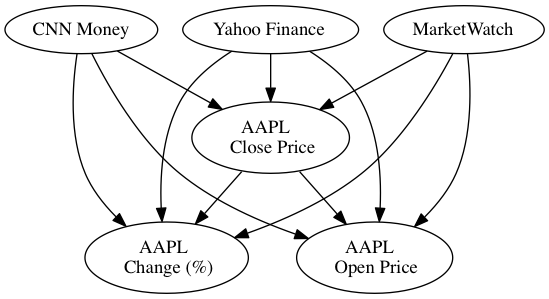
\includegraphics[width=5cm]{bn1.png}
\caption{An example of the attribute dependence model, which models source trustworthiness.}
\label{fig:sourcet}
\end{figure}

\begin{figure}
\centering
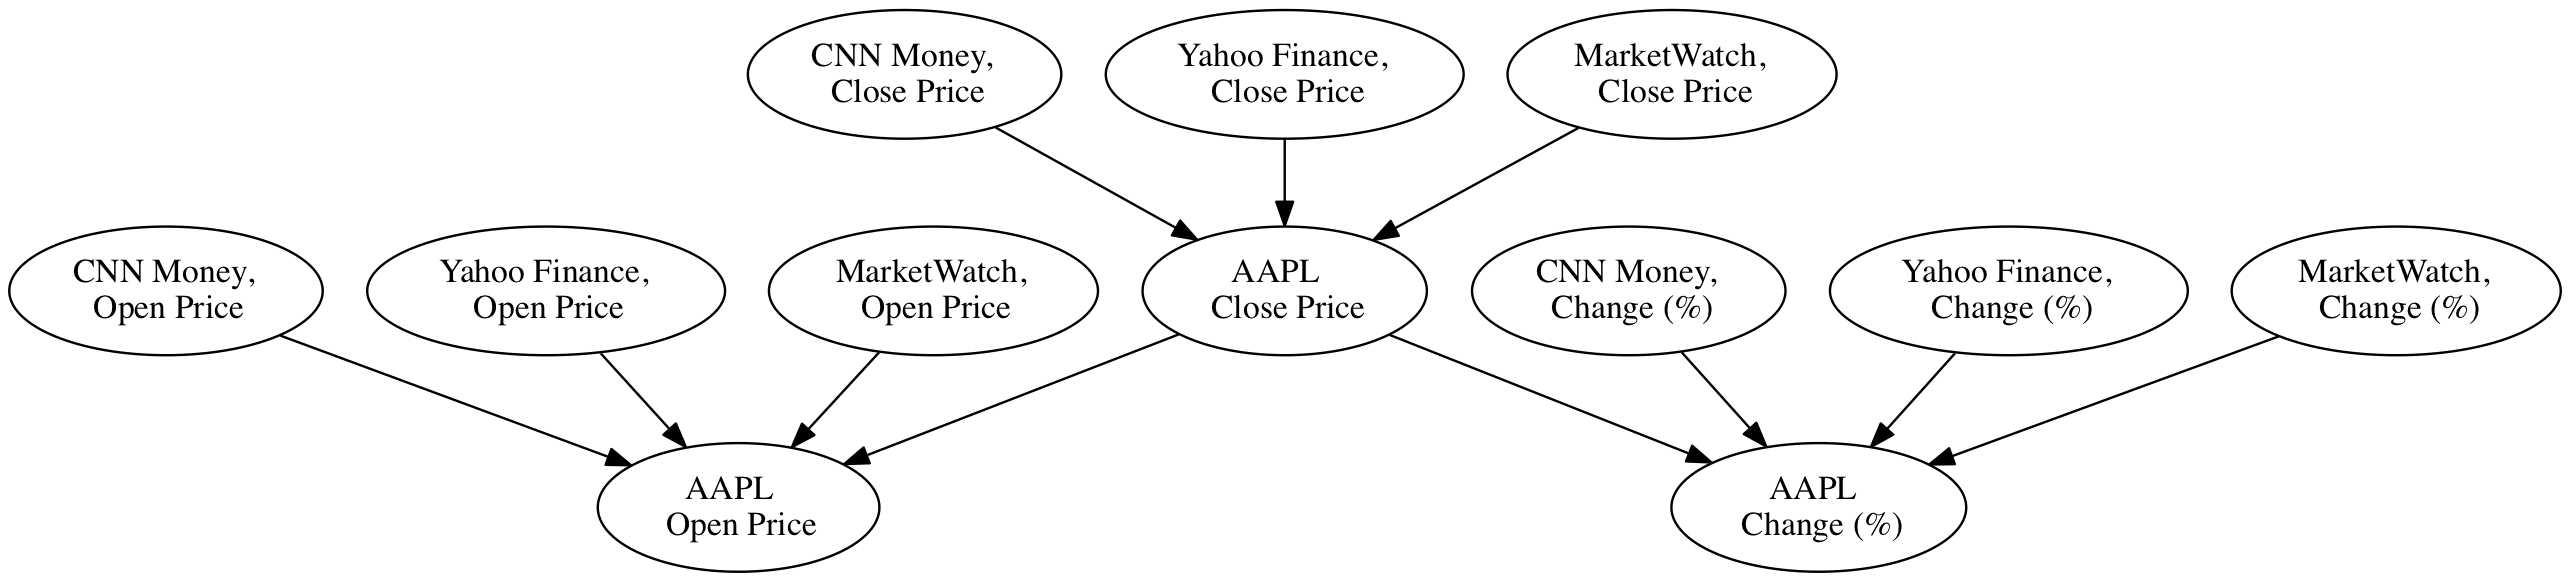
\includegraphics[width=9cm]{bn2.png}
\caption{An example of the attribute dependence model which models the trustworthiness of each attribute provided by a source}
\label{fig:attrt}
\end{figure}

\section{Data Sets} \label{sec:data_sets}


\begin{table*}[t]
\small
\centering
\begin{tabular}{|c|c|c|}
\hline
\textbf{Dataset} & \bf Continuous Attributes & \bf  Categorical Attributes \\
\hline
Book &  & Title, Author names \\
\hline
Stock & Volume, Shares Outstanding, Market Cap & Percent Change, Last Trading Price, Open Price, Change \$, \\
& &  Today's High,  Today's Low, Previous Close, 52wk High, \\
& & 52wk Low,  P/E, Yield, Dividend, EPS \\
\hline
Weather & High Temperature, Low Temperature & Descriptive Condition  \\
\hline
Adult & Age, fnlwgt, capital-gain, & Workclass, education, education-num,  \\
& capital-loss, hours-per-week & marital-status, occupation, relationship, race, \\
& & sex, native-country, income-class \\
\hline
Credit Approval &  A2, A3, A8, A11, A14, A15 & A1, A3, A4, A5, A6, \\
& & A7, A9, A10, A12, \\
& & A13, A16 \\
\hline
\end{tabular}
\caption{Specification of which attributes are continuous and which are categorical}
\end{table*}


\begin{table*}[t]
\small
\centering
\begin{tabular}{|c|c|c|c|}
\hline
\textbf{Dataset} & \bf Numeric Attrs & \bf  String Attrs & \bf Author Name Attrs\\
\hline
Book &  & Title &Author names \\
\hline
Stock & Volume, Shares Outstanding, & &\\
& Market Cap, Percent Change, & & \\
&  Last Trading Price, Open Price, && \\
& Change \$, Today's High, && \\
& Today's Low, Previous Close, && \\
& 52wk High, 52wk Low, && \\
& P/E, Yield, Dividend, EPS & & \\
\hline
Weather &  High Temperature, Low Temperature & Descriptive Condition & \\
\hline
Adult & Age, fnlwgt, capital-gain, & Workclass, education, education-num, & \\
& capital-loss, hours-per-week & marital-status, occupation, relationship, race, &\\
& & sex, native-country, income-class & \\
\hline
Credit Approval &  A2, A3, A8, A11, A14, A15 & A1, A3, A4, A5, A6,  & \\
& & A7, A9, A10, A12,  & \\
& & A13, A16  & \\
\hline
\end{tabular}
\caption{Specification of the data type of each attribute}
\end{table*}

\subsection{Weather Dataset}

In the data obtained from \cite{li:resolving} we could not distinguish between the high and low temperatures and so ended up having a single attribute for temperature. No entity had more than one value for this attribute from a given source and so this is ok. 


\section{Experiments}

\subsection{Data Preprocessing}

The stock and book datasets presented in Section \ref{sec:data_sets} requires additional preprocessing to clean the data before it can be used as input to the fusion algorithms. Schema mapping was applied to the data by the data set creators; each source presents data for the same set of attributes. However, the formatting of attribute values is too diverse and noisy to be used as is.  The {\sc CRH} and {\sc TruthFinder} algorithms include operations measuring the similarity of attribute values. For attributes with numeric values, distance measures such as absolute distance and squared distance are used.  There are values for numeric attributes in the stock dataset which cannot be parsed by Java's built in String to numeric converters, such as $7,453,234$ and $\$45\text{M usd}$. To convert these and other values from strings to numbers, we used a deterministic rule based approach, which matches regular expressions to parse the data. For numeric attributes, we handle four or more digit numbers separated by commas; percentages; monetary figures with text denotations for thousands, millions, and billions of dollars; and scientific notation. The gold data is also provided in this format and the same regular expressions are used to parse it as well. Similarly, algorithms presented in \cite{dong:integrating} and \cite{yin:truth} operate on the \emph{author name} attribute of the book dataset with the structure of first, middle and last names. The dataset is not labeled with this structure and the names are not given in a consistent order of name components. Additionally, lists of authors are not delimited in a consistent way and in fact often do not have delimiters. It was not clear to us how each paper converted the raw text into structured author names. We wrote regular expressions for  11 common arrangements of first, middle and last names (including first and middle initials). We parse the raw text in a greedy fashion, that is we start at the first character in the text string, match the longest regular expression pattern and repeat from the first character after the match. The gold data for the book dataset provides the author names in a consistent format. The code for this processing is available in the GitHub repository for our project\footnote{\tt https://github.com/nmonath/DBProject}. We did our best to make the regular expressions effective without over tuning them to the datasets used for evaluation. The regular expressions were necessary to match the evaluation results presented in the literature; their quality can also have a great impact on system performance. We would suggest authors in the future use a fixed set of regular expressions or provide a preprocessed version of the data so that system performance in the evaluation metrics will not be impacted by the regular expressions. 

\subsection{Attribute Domains and Data Types}

In the following presentation of results, we distinguish between attributes with  \emph{categorical} and \emph{continuous} domains. It is important to note that categorical attributes may still have numeric values. The similarity measure in algorithms such as {\sc TruthFinder} can operate on the numeric values of categorical attributes. The data type of the attribute (i.e. numeric, string, list of author names, etc) as well as the domain (categorical or continuous) will impact how the algorithm is evaluated. 

\subsection{Evaluation Metrics}

Each of the datasets provides a gold or ground truth labeling of the attribute values for a portion of the entities. Following \cite{li:truth,li:resolving,waguih:truth,dong:integrating}, we compare the output of the data fusion algorithms on the same portion of the entities to the gold data. We measure the system performance on categorical attributes using precision, recall, F1 and accuracy and the performance on continuous attributes using  the mean absolute distance and mean normalized absolute distance. 

\subsubsection{Categorical Attribute Evaluation}

Precision and recall are defined in the standard way. We take the predicted output to be the set of records in the result of the algorithm about entities  that appear in the gold data. Precision is the number of correct attribute values in the predicted output divided by the number of values in the predicted output. Recall is the number of correct attribute values in the predicted output divided by the number of values in the gold data. F1 is  geometric mean of precision and recall. 


\begin{equation}
\mathsf {Precision =\frac {\sum_{e \in E}  \sum_{\substack{a_g \in Attr^g(e) \\ a_o \in Attr(e)}} \mathsf{Equal}(a_g,a_o)}{\sum_{e \in E}  |(Attr(e))| }}
\end{equation}


 \begin{equation}
\mathsf {Recall =\frac {\sum_{e \in E}  \sum_{\substack{a_g \in Attr^g(e) \\ a_o \in Attr(e)}} \mathsf{Equal}(a_g,a_o)} {\sum_{e \in E}  |(Attr^g(e))| }}
\end{equation}

where $\mathsf{Equal}$($a_g$,$a_o$) is an indicator function that is 1 if value of $a_g$ is considered to be equal to value of $a_o$  and 0 otherwise.


Accuracy is defined in the exact same way as recall. Furthermore, each algorithm  provides a value for each attribute of each entity and the values for precision and recall will be the same (and so the value of F1 will be the same as well). For these reasons, in the following tables we present only accuracy not precision, recall and F1. Also note that the papers \cite{li:resolving} presents error rate rather than accuracy, error rate is one minus the accuracy. 

\subsubsection{Categorical Attribute Evaluation with Tolerance}

Categorical attributes with numeric values in the stock data set are evaluated with slack in \cite{li:truth}. Consider an entity $e$ with an attribute $a$. Let $V_e(a)$ be the set of values presented by the various sources about the attribute $a$ of entity $e$. The $\mathsf{Equal}$ function in the above equation is defined as:

\begin{align}
\mathsf{Equal}&(a_g,a_o) =\\ \nonumber
&[\alpha_g - \lambda \cdot  \mathsf{Median}(V_e(a_o)) \leq \alpha_o \leq \alpha_g + \lambda \cdot  \mathsf{Median}(V_e(a_o))]
\end{align}

where $\lambda = 0.1$ is a tolerance factor and $\alpha_g$ and $\alpha_o$ are the values of the attribute $a_g$ and $a_o$ respectively. This definition only applies to the categorical attributes in the stock dataset. In all other datasets, the $\mathsf{Equal}$ function is defined as an exact match.

\subsubsection{Continuous Attribute Evaluation}

As presented in \cite{li:resolving}, system performance on continuous attributes is measured by the mean absolute distance and mean normalized absolute distance. Mean absolute distance (MAD) is measured as the average of the absolute distance between the value of each pair of entity $e$ and attribute $a$ in the gold data and predicted data. That is:

\begin{equation}
MAD = \frac{1}{N} \sum_{e \in E} \sum_{a \in Attr(E)} | \alpha_g - \alpha_o |
\end{equation}

where $N$ is the number of entity attribute pairs, $\alpha_g$ is the value in the gold set and $\alpha_o$ is the value in the algorithm output. 

The mean normalized absolute distance (MNAD) is defined in a similar way, except with each distance normalized by the variance of all the distance for that attribute. For an attribute $a$, we define $\sigma^2_a$ to be the variance of the set $\{ abs(\alpha_{e,g}-\alpha_{e,g}) |$ where $\alpha_{e,g}, \alpha_{e,o}$ are values for  $a$ for entity $e \in E$\} 

\begin{equation}
MNAD = \frac{1}{N} \sum_{e \in E} \sum_{a \in Attr(E)} \frac{| \alpha_g - \alpha_o |}{\sigma^2_a}
\end{equation}

\subsection{Hyperparameters}

The data sets do not provide a development set for tuning hyper parameters. The papers in the literature present results on the entire set of data and do not appear to hold out data for tuning. For all of the datasets except the book dataset, adjustments to the hyperparameters  had a minor impact on performance (cite numbers). We tuned the hyperparameters  using a grid search and selected the values which gave performance scores which best matched the work in the literature. 

\subsection{Results}

The gold data for the book dataset provides only the author names for each book. An assignment of author names is considered correct only if the authors  match the gold data in first and last name (ignoring middle). The book dataset measures how accurately Regarding the books dataset we nearly match the accuracy of {\sc TruthFinder } to the number presented in \cite{dong:integrating}. We present a value of $0.84$ and \cite{dong:integrating} gives a value of $0.83$. This could be caused by changes in hyperparameters or the preprocessing/parsing of the author names. As there are only 100 records in the gold data, our implementation differs by only one record from the published number. 

The paper \cite{li:truth} presents results on a single day, July 7, 2011, of the stock dataset. Other papers such as \cite{li:resolving} evaluate on every day of the stock dataset. We present results on both the single day and the entire data set. 
\definecolor{shadecolor}{rgb}{0.82,0.82,0.82}
\definecolor{tableShade}{gray}{0.9}
\colorlet{tableheadcolor}{black!90} % Table header colour = 25% gray
\newcommand{\headcol}{\rowcolor{tableheadcolor}} %
\rowcolors{3}{tableShade}{white}  %% start alternating shades from 3rd row

\begin{table*}[t]
\centering
\begin{tabular}{|c|c|ccc|ccc|ccc|}
\hline
\headcol \color{white} Algorithm & \multicolumn{10}{|c|}{  \color{white} Dataset} \\
\hline
\headcol &  \color{white} {Book} & \multicolumn{3}{c}{  \color{white} Single Day Stock}  & \multicolumn{3}{|c|}{ \color{white} Entire Stock} & \multicolumn{3}{|c|}{ \color{white}  Weather }\\
\hline
\headcol &  \color{white} Acc. &  \color{white} Acc. &  \color{white} MAD &  \color{white} MNAD &  \color{white} Acc. &  \color{white} MAD &  \color{white} MNAD & \color{white} Acc. &  \color{white} MAD &  \color{white} MNAD \\
\hline
 Majority Voting & \\
 Mean & \\
 Median & \\
\sc TruthFinder & \\
\sc 2-Estimates & \\
\sc 3-Estimates & \\
\sc CRH & \\
\hline 
\hline
\sc ModifiedTruthFinder & \\
\sc ModifiedCRH & \\
\sc Ensemble & \\
\hline
\end{tabular}
\caption{Results on Real World Datasets}
\label{tbl:vars}
\end{table*}

\begin{table*}[t]
\centering
\begin{tabular}{|c|ccc|ccc|ccc|}
\hline
\headcol \color{white} Algorithm & \multicolumn{9}{|c|}{  \color{white} Dataset} \\
\hline
\headcol &  \multicolumn{3}{c}{  \color{white} Adult}  & \multicolumn{3}{c}{  \color{white} Credit Approval}  & \multicolumn{3}{|c|}{ \color{white} Pima Indians Diabetes} \\
\hline
\headcol &  \color{white} Acc. & \color{white} MAD &  \color{white} MNAD &  \color{white} Acc. &  \color{white} MAD &  \color{white} MNAD & \color{white} Acc. &  \color{white} MAD &  \color{white} MNAD \\
\hline
 Majority Voting & \\
 Mean & \\
 Median & \\
\sc TruthFinder & \\
\sc 2-Estimates & \\
\sc 3-Estimates & \\
\sc CRH & \\
\hline 
\hline
\sc ModifiedTruthFinder & \\
\sc ModifiedCRH & \\
\sc Ensemble & \\
\hline
\end{tabular}
\caption{Results on Synthetic Datasets}
\label{tbl:vars}
\end{table*}


\subsection{Initial Experiments}

\subsubsection{Upperbound}

\subsubsection{Best Sources per Dataset}


\section{Discussion}

\subsection{Source Trustworthiness}


\bibliographystyle{abbrv}
\bibliography{references}  

\balancecolumns
\end{document}
